\documentclass[a4paper,12pt, projekat]{etf}

\usepackage[intlimits]{amsmath}
\usepackage{amsmath, amsfonts, amssymb, graphicx}

\usepackage[serbian]{babel}
\usepackage[T1]{fontenc}
\usepackage[utf8]{inputenc}

\addto\captionsserbian{\renewcommand{\bibname}{Literatura}}

\title{Prepoznavanje stanja industrijske tastature kori\v{s}\'{c}enjem openCV
biblioteke}
\author{Lazar Caković}
\indeks{3083/2016}
\date{jul 2018.}
\mentor{prof.~dr Nenad Jovi\v{c}i\'{c}; as. Ms. Marija Jankovi\'{c}}
\predmet{Ma\v{s}inska vizija}

\begin{document}

	\maketitle

	\tableofcontents

	\listoffigures

	\newpage

	\chapter{Uvod}
        Cilj projekta iz predmeta Ma\v{s}inska vizija, na master studijama odseka
        za Elektroniku, bio je da se na tastaturi koja se koristi u industrijske
        svrhe detektiju stanja same tastature kori\v{s}\'{c}enjem kamere koja je javno
        dostupna, kao i da se manipulacijom stanja tastature, prepoznavanje
        kamere prilagodi tako da uvek daje informacije o stanju koje odgovaraju
        trenutnom stanju na samoj kameri. Realizacija projekta je odradjena tako
        da se lako moze iskoristiti u sklopu ve\'{c}eg sistema, tako da informacije
        prikupljene uz pomo\'{c} ovog programa mogu biti iskori\v{s}\'{c}ene u nekoj daljoj
        obradi.

        \begin{figure}[htb]
            \centering
            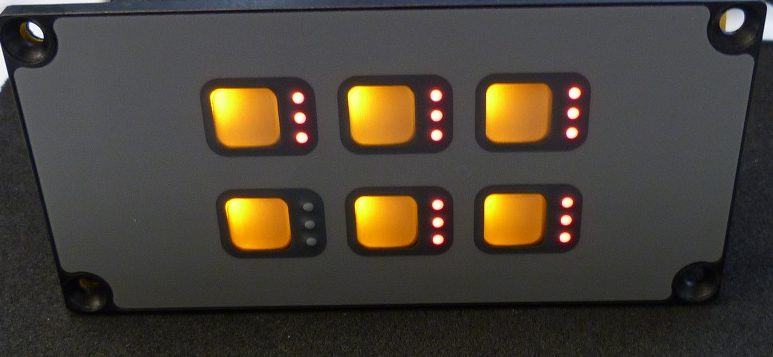
\includegraphics[scale=.5]{front.jpg}
            \caption{Pogled na tastaturu odozgo}
            \label{fig:keyboard}
        \end{figure}

        \chapter{Opis sistema}
        Tastatura koja je kori\v{s}\'{c}ena pri izradi projekta je industrijska tastatura
        koja se koristi u velikim gradjevinskim ma\v{s}inama. Sama tastatura ima 6
        tastera, rasporedjenih u 3 reda, jedan ispod drugog, po dva u redu. I
        iznad svakog tastera postoje 3 diode. Diode koje se nalaze iznad
        tastera predstavljaju trenutno stanje na izlazu same tastature, a kao
        reakcija na trenutno stanje u nekom ve\'{c}em sistemu, i kao reakcija na
        sam pritisak tastera na tastaturi. Kako je emulacija celokupnog sistema
        u kome radi tastatura previse kompleksna, za izradu projekta je
        kori\v{s}\'{c}ena jednostavnija postavka. Tastaura ima ulazne i izlazne pinove
        preko kojih je mogu\'{c}e komunicirati sa samom tastaturom. Interfejs preko
        kog se kontroli\v{s}e tastatura je CAN interfejs. I na osnovu slanja
        odredjenih poruka preko CAN interfejsa mogu\'{c}e je kontrolisati koje
        diode su uklju\v{c}ene, odnosno isklju\v{c}ene. I takodje, u kom
        re\v{z}imu \'{c}e sama tastatura raditi. Za realizaciju samog projekta,
        tastatura je pode\v{s}ena tako da se slanjem odredjenih poruka, menja stanje
        dioda na tastaturi, \v{c}ija je stanja potrebno prepoznati. S ovim u
        vezi, kori\v{s}\'{c}en je konverter USB/CAN i program proizvodja\v{c}a samog
        konvertera kako bi se slale CAN poruke ka tastaturi.

        \begin{figure}[htb]
            \centering
            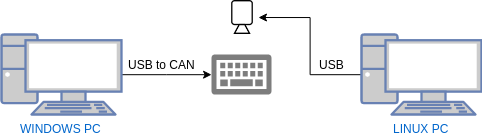
\includegraphics[scale=0.5]{keyboardSetup.png}
            \caption{Prikaz postavke sistema}
            \label{fig:keyboardsetup}
        \end{figure}

        Slanjem razli\v{c}itih poruka menjaju se stanja dioda, \v{c}ime se testira
        algoritam za prepoznavanje trenutnog stanja. Kamera koja je
        kori\v{s}\'{c}ena prilikom izrade projekta je USB Web kamera.

        \begin{figure}[htb]
            \centering
            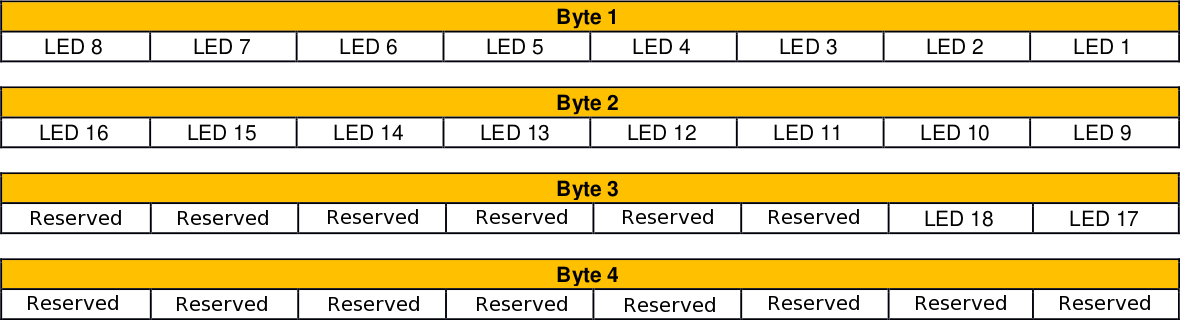
\includegraphics[scale=0.3]{canmsg.png}
            \caption{Prikaz CAN poruke prema tastaturi za manipulaciju diodama}
            \label{fig:keyboardmsg}
        \end{figure}

        \chapter{Softverska implementacija}
        Softverska implementacija projekta je odradjena u programskom jeziku
        Python uz kori\v{s}\'{c}enje biblioteke openCV za obradu slike.

        Implementacija je podeljena u dva dela, kalibraciju scene i dela za
        procesiranje trenutne slike koja se dobija sa kamere. Implementacija je
        napravljena tako da snimci sa pocetka pokretanja programa vrse
        kalibraciju, nakon cega sa podacima koji su dobijeni u kalibraciji
        dolazi do dela za procesiranje.

        \section{Deo za kalibraciju}
        Kako bi se odradila kalibracija na pocetku, potrebno je da se tastaturi
        po\v{s}alje komanda o uklju\v{c}enim svim diodama iznad tastera. I to iz
        razloga pozicioniranja svih dioda u sistemu, odnosno svesti programa o
        poziciji svih dioda koje se nalaze na tastaturi. Unutar dela za
        kalibraciju vr\v{s}i se obrada slike u nekoliko koraka. Prvo se vr\v{s}i
        pretvaranje slike u crno-belu sliku, s obrzirom da boja dioda ne igra u
        ovom algoritmu nikakvu ulogu. S tim da se i to moze iskoristiti
        prilikom nekih slo\v{z}enijih algoritama za odredjivanje trenutnog stanja
        tastature. Nakon toga se vrsi ekvalizacija histograma i fitriranje
        Gausovim filtrom 5 reda. I binarizacija sa odredjenim pragom, kako bi
        se samo sjaj dioda izdvojio na slici u beloj boji. Pri \v{c}emu je prag
        binarizacije odredjen emprijski, s obzirom da tasteri koji se nalaze
        ispod dioda imaju pozadinsko osvetljenje, koje u ovom projektu nije od
        interesa za odredjivanje stanja dioda. Na kraju, koristi se funkcija
        HoughCircles za odredjivanje obrazaca iz biblioteke openCV\@. Ova
        funkcija nalazi krugove zadatog pre\v{c}nika na crno-beloj slici. Takodje,
        uz zadat pre\v{c}nik, potrebno je zadati jos neke parametre kako bi se
        krugovi na slici odredili u najve\'{c}em broju slu\v{c}ajeva. Ova funkcija je
        iskori\v{s}\'{c}ena zbog same postavke kamere u odnosu na tastaturu, kao i
        samog oblika dioda koje se poku\v{s}avaju odrediti. Kako je cela postavka
        fiksna, empirijski su odredjene vrednosti koje se prosledjuju kao
        argumenti funkciji za odredjivanje krugova. Kada se dobiju svi krugovi
        koji se nalaze na samoj tastaturi, onda se prelazi na sortiranje
        nadjenih rezultata, i to tako da se u nizu prvo nalazi prvi red dioda,
        pa drugi, i na kraju tre\'{c}i, sa koordinatama centara dioda. Kalibracija
        se zavr\v{s}ava kada se 10 puta pronadju svih 18 dioda na tastaturi. Broj
        ta\v{c}nih odredjivanja je uzet proizvoljno. Nakon zavr\v{s}etka odredjivanja
        dioda u kalibraciji, dolazi do usrednjavanja vrednosti koje su
        dobijene, i to tako da se dobiju sigurne pozicije dioda nakon
        kalibracije, odnosno centri krugova koji predstavljaju diode.

        \section{Deo za procesiranje}
        Nakon dela za kalibraciju, vrsi se procesiranje ulazne slike na osnovu
        podataka koji su dobijeni iz dela za kalibraciju. Ovaj deo softverske
        implementacije se odnosi na deo za detekciju okulzije, i ostatka
        procesiranja. Detekcija okulzije se vrsi funkcijama za odredjivanje
        pomeraja na osnovu pozadine. Prilikom pravljenja maske za odredjivanje
        pomeraja na osnovu pozadine koristi se trenutna slika koja je dobijena
        sa kamere u tom trenutku. Na osnovu \v{c}ega se koriste funkcije za
        statisti\v{c}ku obradu slike, za pomeraj koji je odredjen, odakle se
        dobijaju kordinate pravougaonika u kome se nalazi objekat koji je usao
        u trenutnu scenu. Ukoliko ovaj deo obrade da neke rezultate, odnosno
        ukoliko se detektuje neki strani objekat na sceni, pauzira se sa
        detekcijom stanja dioda sve dok se objekat ne ukloni. Nakon cega se
        detekcija nastavlja. Detekcija se odvija samo ukoliko ne postoje
        smetnje, i ona se odvija u delu preprocesiranja koje se sastoji od
        istih koraka kao u kalibraciji, odnosno jednostavnih metoda za obradu
        slike, pri cemu je zavr\v{s}ni korak dobijanje binarizovane slike. Kako su u
        kalibraciji dobijene sve pozicije dioda, iz binarizovane slike je
        moguce odlu\v{c}iti o stanju dioda samo jednostavnim upitom da li je piksel
        na poziciji centra odredjenog kruga nula ili jedan. Time se dobija
        trenutno stanje dioda. Kako su podaci iz kalibracije sortirani po
        redovima i pozicijama dioda, onda je vrlo lako napraviti odlu\v{c}ivanje o
        trenutnom stanju. U ovom delu se takodje i ispisuju sve relevantne
        poruke na standardni izlaz, kako bi korisnik imao uvid u to kako
        program radi.

        \chapter{Apendix}

\begin{verbatim}

import os
import cv2
import numpy as np
import pdb

def calibration(cap, count):
    # getting one frame from camera input
    ret, frame = cap.read()
    circles = np.zeros([18,3], dtype=int)
    # switch to gray image
    grayImg = cv2.cvtColor(frame, cv2.COLOR_BGR2GRAY)
    # equilize histogram
    modifiedImg = cv2.equalizeHist(grayImg)
    # smoth equilized image
    smothedImg = cv2.GaussianBlur(modifiedImg, (5, 5), 1.5)
    # get only brightest parts of image
    ret,binImg = cv2.threshold(grayImg, 200, 255, cv2.THRESH_BINARY)
    # find circles in binarized image
    circles = cv2.HoughCircles(binImg,cv2.HOUGH_GRADIENT,1,18,
            param1=200,param2=10,minRadius=5,maxRadius=10)

    if circles is not None:
        circles = np.uint16(np.around(circles[0]))
        if circles.shape[0] == 18:
            circles = circles[circles[:,0].argsort()]
            circlesFirst = circles[:6]
            circlesFirst = circlesFirst[circlesFirst[:,1].argsort()]
            circlesSecond = circles[6:12]
            circlesSecond = circlesSecond[circlesSecond[:,1].argsort()]
            circlesThird = circles[12:]
            circlesThird = circlesThird[circlesThird[:,1].argsort()]
            circles = np.vstack((circlesFirst, circlesSecond, circlesThird))
            count = count + 1
    else:
            circles = np.zeros([18,3], dtype=int)

return frame,count,circles


### Live stream
cap = cv2.VideoCapture(0)

### Added for substraction
# make structuring element for morph transformation of substracted image
# MORPH_OPEN with MORPH_ELLIPSE, to kill all noise from MOG2 substraction
# (errosion, then dilation), with this killed all noise
kernel = cv2.getStructuringElement(cv2.MORPH_ELLIPSE, (3,3))
# getting the changes from live image in comparison with background created
# with MOG2 here. applying the subtractor after every frame taken in loop
fgbg = cv2.bgsegm.createBackgroundSubtractorMOG()
### Added for substraction

count = 0
i = 0
mode = 1

if mode == 0:
    while(True):
        ### Testing mode
        # only for showing the image from camera, only made for positioning
        # the camera
        ret, frame = cap.read()

        cv2.imshow('frame', frame)
        if cv2.waitKey(1) & 0xFF == ord('q'):
            break
else:
    circlesAll = np.zeros([18,3], dtype=int)
    diodeState = np.zeros([18,1], dtype=int)

    print("Calibration started...")
    while(True):

        ### calibration part
        while count<10:
            frame, count, circlesTemp = calibration(cap, count)
            if circlesTemp.shape[0] == 18:
                circlesAll += circlesTemp

        if count == 10:
            print("Calibration ended...")
            circlesAll = np.uint16(np.around(circlesAll/10))
            print(circlesAll)
            count = 100

        # getting one frame from camera input
        ret, frame = cap.read()

        # use substractor on current frame, and morph on substracted image
        fgmask = fgbg.apply(frame)
        fgmask = cv2.morphologyEx(fgmask, cv2.MORPH_OPEN, kernel)
        # find contour features and draw rectangle if there is something
        output = cv2.connectedComponentsWithStats(fgmask, 4, cv2.CV_32S)
        for i in range(output[0]):
            if output[2][i][4] >= 8000 and output[2][i][4] <= 100000:
                cv2.rectangle(frame, (output[2][i][0], output[2][i][1]),
                        (output[2][i][0] + output[2][i][2],
                        output[2][i][1] + output[2][i][3]),
                        (0, 255, 0), 2)

        if output[0] == 1:
            ### processing part
            # if there are no intrusions in current scene
            # make gray image
            grayImg = cv2.cvtColor(frame, cv2.COLOR_BGR2GRAY)
            # equilize histogram
            modifiedImg = cv2.equalizeHist(grayImg)
            # smoth equilized image
            smothedImg = cv2.GaussianBlur(modifiedImg, (5, 5), 1.5)
            # get only brightest parts of image
            ret,binImg = cv2.threshold(grayImg, 200, 255, cv2.THRESH_BINARY)
            os.system('clear')

            print("    ROW  |   COL   |   VALUE")
            # ask for
            for i in range(0, 18):
                # ask for every found diode is it white or black (on or off)
                if binImg[circlesAll[i][1],circlesAll[i][0]] == 255:
                    diodeState[i] = 1
                else:
                    diodeState[i] = 0
                row, col = divmod(i, 6)
                print("   ", row+1, "   |   ", col+1, "   |  ", diodeState[i])

            ### drawing positions of diodes calibration have found
            for i in circlesAll[:]:
                # draw the outer circle
                #  cv2.circle(frame,(i[0],i[1]),i[2],(0,255,0),2)
                # draw the center circle
                cv2.circle(frame,(i[0],i[1]),1,(0,0,255),2)
        else:
            os.system('clear')
            print("Intrusion detected!")

        cv2.imshow('frame', frame)
        if cv2.waitKey(1) & 0xFF == ord('q'):
            break

cap.release()
cv2.destroyAllWindows()

\end{verbatim}

\end{document}
